\section{Concrete implementation}
\label{sec:concrete}

\newcommand{\con}[1]{\ensuremath{{\color{red} #1}}}
\newcommand{\abs}[1]{\ensuremath{{\color{blue} #1}}}

The operational semantics we have defined in the previous section
satisfy non-interference by design.
We achieve this general statement that works for a large class of
languages by having different task execute completely isolated from
each other, such that every task has its own state.
In some cases, this strong separation is desirable, or even necessary.
Languages like C provide direct access to memory locations without
mechanisms in the language to achieve a separation of the heap.
On the other hand, for other languages this
strong isolation of tasks can be
undesirable, e.g., for performance reasons.
For instance, for the language |targetLangML|, our presentation so far
requires a separate heap per task, which is not very practical.
Instead, we would like to
more tightly couple the integration of the target and IFC
language by reusing existing infrastructure.  In the running example,
a concrete implementation might use a single global heap.
More precisely, instead of using a configuration of the form
\[|iconf iS (fullconf id1 il1 tS1 ie1, fullconf id2 il2 tS2 ie2 ldots)|\]
we would like a single global heap as in
\[|oneheapiconf iS tS (oneheapfullconf id1 il1 ie1, oneheapfullconf id2 il2 ie2, ldots)|\]

If the operational rules are adapted na\"ively to this new setting,
then non-interference can be violated.  In particular, it is not
sound to share references to a heap cell between different tasks.
Otherwise, information can be trivially leaked by copying
secret data into a reference in one task, and then
reading it again by a another task with a lower label.
Clearly, we cannot
modify the semantics in arbitrary ways if we are hoping to preserve
non-interference, but how can we know if our changes to the abstract
semantics preserve non-interference?
The intention of our single heap implementation was to be more efficient
by using one global heap, but conceptually maintain isolation between
task by not allowing sharing of references between tasks.
This intuition of having a different (potentially more efficient)
concrete semantics that behave like the abstract semantics
can be formalized by the following definition:

\Red{We really should not use red/blue here.  I suggest we just use primes instead of colors here.}
\begin{definition}[Isomorphism of information-flow control languages]
  A language \con{|(C, .->, erasef l)|} is \textit{isomorphic} to a
  language \abs{|(iC, .->, erasef l)|} if there exist total functions |f
  : tC -> iC| and |finv : iC -> tC| such that |f .. finv = idf tC| |finv
  .. f = idf iC|.  Furthermore, |f| and |finv| are functorial (e.g. if
  $\abs{x\ R\ y}$ then $f(\abs{x})\ \con{R}\ f(\abs{y})$) over both
  $l$-equivalences and |.->|.
  
  If we weaken this restriction such that |finv| does
  not have to be functorial over |.->|, we call the
  language \con{|(C, .->, erasef l)|} \textit{weakly isomorphic} to
  \abs{|(iC, .->, erasef l)|}.
\end{definition}

Providing an isomorphism between the two languages allows us to
preserve (termination sensitive or insensitive) non-interference
as the following two theorems state.

\begin{theorem}[Isomorphism preserves termination sensitive non-interference]
  \label{thm:iso-tsni}
  If \ifc{L} is isomorphic to \tar{L} and \ifc{L} satisfies TSNI, then
  \tar{L} satisfies TSNI.
\end{theorem}

\begin{proof}
  Shown by transporting configurations and reduction derivations from
  \tar{L} to \ifc{L}, applying TSNI, and then transporting the
  resulting configuration, $l$-equivalence and multi-step derivation back.
\end{proof}

\begin{theorem}[Weak isomorphism preserves termination insensitive non-interference]
  \label{thm:iso-tini}
  If a language \con{L} is weakly isomorphic to a language \abs{L}, and \abs{L}
  satisfies TINI, then \con{L} satisfies TINI.
\end{theorem}

\begin{proof}
  Shown by transporting configurations and reduction derivations
  from \con{L} to \abs{L}, applying TINI and transporting the resulting
  equivalence back using functoriality of |finv| over $l$-equivalences.
\end{proof}

A na\"ive attempt at our single heap semantics
will not allow us to construct an isomorphism
with the abstract language |specLangML alpha|, and instead highlights
where things will go wrong.
To successfully construct an isomorphism, our concrete semantics need
to mirror the behavior of the abstract semantics, most importantly
in the case where tasks interact.  Namely, at a fork and when sending
or receiving messages, we take an expression from one task and
execute it in the context of another task.  In the abstract semantics
the fork rule is parameterized by the strategy |klone|, which defines
what heap the new task should execute in.  \Red{In Section~\ref{sec:retrofit}
we have motivated two choices}, namely the identity (to effectively
clone the heap), or to start with an empty heap.
In the latter case, this effectively means that existing addresses
in the forked expression |ie| are no longer valid and the
task gets stuck (and then removed by \textsc{I-noStep}).
\todo{}{Is this actually true?  Currently the semantics are unclear.}
To get the isomorphic behavior in the concrete semantics with a
single heap, we would have to change the forked expression |ie| in
such a way that all addresses get rewritten to fresh addresses
that are guaranteed to not occur in the global heap.  Similarly,
sending a memory address should take a similar approach, as addresses
for sent references will not exist in the receiving task.

If |klone| is the identity function, then the abstract semantics
effectively clone the heap on a fork.  To get an isomorphic
behavior in the concrete, we would have to create a copy of everything
reachable from the forked expression (not just the values for
the memory addresses in the expression), and replace all addresses
correspondingly.  Even worse, the behavior of sending a memory address
now depends on whether that address existed at the time the receiving
task was forked;  if it did, then the address should be rewritten to the
new one, otherwise to a fresh address.
Such a complicated behavior is contradictory to our initial motivation
of implementing a single heap for efficiency.  But also the
behavior of the simpler case where |klone| returns an empty heap is
undesirable:  We rewrite addresses to fresh addresses, which will
result in a stuck task whenever such an address is dereferenced.

\subsection{Restricting the IFC Language}

As a better solution we could forbid forked expressions as well
as messages sent to other tasks to contain memory addresses in the
first place.  In a statically typed language, the type system could
prevent this from happening, and we talk more about how our
approach integrates with typed languages in
Section~\ref{sec:extensions:types}.
In a dynamically type languages such as |targetLangML|, we might
restrict the transition for |fork| and |send| to only allow expressions
without memory addresses.

Again we are modifying the IFC language semantics in a non-trivial way,
which begs the question whether non-interference is preserved.
Note that restricting the transitions in an information flow control
system in general does not preserve non-interference as the following
minimal example illustrates.
Consider a trivial state machine as shown
in Figure~\ref{fig:trivial-sm}, whose second projection is classified
secret.  With all three transitions, this language fulfills
termination sensitive non-interference.  Furthermore, if the
dashed transition
is removed, the language continues to satisfy TSNI.  However, if any
solid line is removed, the language fails TSNI.

\begin{figure}
  States: $(x,y)$ for $x,y \in \{0,1\}$ \\
  Erasure function: $f(x,y) = (x,\bullet)$
  
  \begin{center}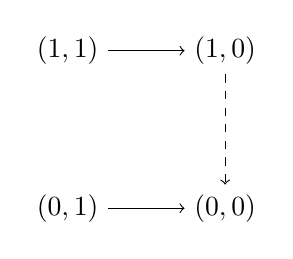
\begin{tikzpicture}[node distance=2cm, auto]
    \node (A) {$(1,1)$};
    \node (B) [right of=A] {$(1,0)$};
    \node (C) [below of=A] {$(0,1)$};
    \node (D) [right of=C] {$(0,0)$};
    \draw[->] (A) to node {} (B);
    \draw[->] (C) to node {} (D);
    \draw[->, dashed] (B) to node {} (D);
    \end{tikzpicture}\end{center}
  
  \label{fig:trivial-sm}
  \caption{A trivial state machine}
\end{figure}

To remedy this issue, we give a definition that gives a condition
under which it is safe to restrict the abstract IFC language
|specLang alpha targetLang|, such that non-interference is preserved.

\begin{definition}[Restricted IFC language]
  \label{def:restricted}
  For a family of predicates $\mathcal P$ (one for every reduction
  rule), we call
  |restrictedLang alpha targetLang| a restricted IFC language
  if its definition is equivalent to the abstract language
  |specLang alpha targetLang|, with the following exception:
  The reduction rules are restricted
  by adding a predicate $P$ from $\mathcal P$ to the premise of
  all rule other than \textsc{I-noStep}.  Furthermore, the predicates $P$
  can depend only on the \textit{erased} configuration
  |erase il ic|, where |il| is the label of the first task
  in the task list and |ic| the full configuration.
\end{definition}

By the following theorem, the restricted IFC language with an
appropriate scheduling policy is non-interfering.

\begin{theorem}
  \label{thm:restricted}
  For any target language |targetLang| and family of predicates
  $\mathcal{P}$, the IFC language |restrictedLang roundrobinf targetLang|
  is TSNI.  Furthermore, the IFC language
  |restrictedLang seqf targetLang| is TSNI.
\end{theorem}


\subsection{IFC language with a single heap}

We are now ready to make our single heap IFC language precise and
ensure its non-interference using the techniques presented.
First, we can construct the restricted language
|restrictedLangNoRef alpha targetLangML|, where |noRefs| is
the family of always valid predicates, except for the ones for
\textsc{I-fork} and \textsc{I-send}, which we define as
\[ P = \text{|ie| does not contain any address |ta|} \]
That is, we do not restrict any rules except for \textsc{I-fork}
and \textsc{I-send}.
Since $P$ only depends on |ie|, which is part of the current
task and thus never erased w.r.t.\ the label of the first task,
this language satisfies non-interference by Theorem~\ref{thm:restricted}.

\begin{figure}
  
  \begin{mathpar}
    \inferrule[C-fork]
    {
      \text{|ie| does not contain any |ta|}\\
      |iS' = iS [ id' mapsto nil ]|\\
      |it1 = oneheapfullconf id il (iniE id')|\\
      |itnew = oneheapfullconf id' il (TI ie)|\\
      |fresh (id')|
    }
    {|
      oneheapiconf iS tS (oneheapfullconf id1 il1 (iniEi (fork ie)), ldots)
      .->
      iS'; tS; sched F (it1, ldots, itnew)
    |}
    \and
    \inferrule[C-send]
    {
      \text{|ie| does not contain any |ta|}\\
      |il canFlowTo il'|\\
      |iS(id') = Q|\\
      |iS' = iS [ id' mapsto (il', id,  ie) , Q ]|
    }
    {|
      oneheapiconf iS tS (oneheapfullconf id il (iniEi (send id' il' ie)), ldots)
      ->
      iS; tS; sched step (oneheapfullconf id il unit, ldots)
    |}
  \end{mathpar}
  
  \caption{A selection of the reduction rules for |concreteLangMl alpha|.}
  \label{fig:concrete}
\end{figure}

The essential parts of the semantics for the concrete language
with a single heap,
which we call |concreteLangMl alpha|,
are given in Figure~\ref{fig:concrete}.  Most rules are
straight-forward translations of the rules in Figures~\ref{fig:ifc}
and~\ref{fig:embedding} but for a single heap.  For conciseness, we
only show the interesting ones.
Now, we can show an isomorphism between this language and
|restrictedLangNoRef alpha targetLangML|, which
(by Theorem~\ref{thm:iso-tsni} and~\ref{thm:iso-tini}) guarantees
non-interference for an appropriate scheduling policy |alpha|.

\Red{Show the isomorphism.}


\section{Proofs}
\label{sec:proofs}

In this section we will prove all theorems we have stated so far.
We observe that the non-interference claims for the languages
|specLang seqf targetLang| and |specLang roundrobin targetLang|
in Theorems~\ref{thm:rr-tsni} and~\ref{thm:seq-tini} follow directly
from Theorems~\ref{thm:iso-tsni} and~\ref{thm:iso-tini},
respectively, about restricted IFC languages where the set
of predicates is the set of always valid predicates.

Before we proceed with the proof of Theorem~\ref{thm:iso-tsni},
we state a lemma we will use.

\begin{lemma}
  \label{lemma:rr-tsni-general}
  We consider, for any target language |targetLang|,
  the restricted IFC language |restrictedLang alpha targetLang|
  (according to Definition~\ref{def:restricted}).
  Then,
  for any configurations |ic1|, |ic1'|, |ic2|, and label |il| where
  \begin{equation} \label{eq:tsni-lemma-lhs}
  |ic1| \approx_{|il|} |ic2|
  \qquad \text{and} \qquad
  |ic1| |.->| |ic1'|
  \end{equation}
  there exists a configuration |ic2'| such that
  \begin{equation} \label{eq:tsni-lemma-rhs}
  |ic1'| \approx_{|il|} |ic2'|
  \qquad \text{and} \qquad
  |ic2| |.->|^* |ic2'|
  \ \text{.}
  \end{equation}
\end{lemma}

\begin{proof}[Proof of Theorem~\ref{thm:iso-tsni}]
  We proof the theorem by induction on the length of the derivation sequence in~\eqref{eq:tsni-lhs}.
  The base case for derivations
  of length 0 is trivial, allowing
  us to simple chose $|ic2'=ic2|$.  In the step case, we assume
  the theorem holds for derivation sequences of length up to $n$, and show that it also
  holds for those of length $n+1$.  We split the derivation sequence from~\eqref{eq:tsni-lhs} as follows:
  \[
  |ic1| |.->| |ic1''| |.->|^n |ic1'|
  \]
  for some configuration |ic1''|.  By Lemma~\ref{lemma:rr-tsni-general}, we get
  |ic''| with
  \begin{equation} \label{eq:tsni-proof-1}
  |ic1''| \approx_{|il|} |ic2''|
  \qquad \text{and} \qquad
  |ic2| |.->|^* |ic2''|
  \end{equation}
  Applying the induction hypothesis to
  $|ic1''| |.->|^n |ic1'|$, we get |ic2'| with
  \begin{equation} \label{eq:tsni-proof-2}
  |ic1'| \approx_{|il|} |ic2'|
  \qquad \text{and} \qquad
  |ic2''| |.->|^* |ic2'|
  \end{equation}
  Stitching together the derivation sequences from~\eqref{eq:tsni-proof-1} and~\eqref{eq:tsni-proof-2} directly gives
  us the right-hand side of the implication in the TSNI
  definition~\eqref{eq:tsni-rhs}, which concludes the proof.
\end{proof}
\begin{proof}[Proof of Lemma~\ref{lemma:rr-tsni-general}]
  First, we observe there must be at least one task in |ic1|, otherwise
  it could not take a step.  Thus, |ic1| is of the form
  |iconf iS1 (it1, its1)|.  Consider two cases:
  \begin{itemize}
    \item $|erase il it1|=|bullet|$.
    By the definition of |erasef il|, we know that |il canFlowTo lcurr|
    where |lcurr| is the label of |it1|.
    In this case, we do not need to take a step for
    |ic2|, because |ic2'=ic2| will already be |il|-equivalent to |ic1'|.
    To see that, note that the tasks |its1| in |ic1| are left in the
    same order and unmodified (the scheduling policy only
    modifies the first task). The task |it1| either
    gets dropped (by \textsc{I-noStep}), or
    transforms into a task |it1'| as well as potentially spawning a new
    task |it1''|.  Since both |it1'| and |it1''| have a label that is
    at least as high as the label of |it1| (can be seen
    by inspecting all reduction rules), they will get filtered
    by |erasef il| in |ic1'|.  Therefore, the |il| equivalence of the
    task list is guaranteed.
    Lets consider the possible changes to |iS1|:
    Only three reduction rules change |iS1|,
    thus it suffices to consider these cases:
    \begin{description}
      \item[Case \textsc{I-send}]
      A new message triple with label |il'| gets added to the message
      queue of the receiving thread.  However, since |lcurr canFlowTo il'|,
      the triple will get erased.
      \item[Case \textsc{I-recv} and \textsc{I-noRecv}]
      In this case, only the queue of
      task |it1| can change, which gets erased.
    \end{description}
    This ensures that $|ic1'|\approx_{|il|}|ic2'|=|ic2|$.
%    \alphacondition{We need all scheduling policies to not change the order
%      of any tasks (except for the first one).  Newly spawned task can appear
%      anywhere in the list.}
    \item $|erase il it1|\neq|bullet|$.
    Here, there must be a corresponding
    task |it2| in |ic2|,
    such that |it1=it2| (otherwise |ic1| and
    |ic2| could not be |il| equivalent).
    However, |it2| might not be at the beginning of the task list yet, but
    all tasks occurring before it must get erased by |erasef il|.
    In |ic2|, we can first take some number of steps until |it2| moves
    to the front of the list.
    This is the case regardless of any additional side conditions $P$ on
    rules, because for all of these tasks, it can either take an actual
    step, or it gets dropped by \textsc{I-noStep} (which is always
    possible, as there cannot be an additional side condition on this
    rule).  All tasks that didn't get dropped are still at a label
    that isn't below |il| and thus get erased.
    
%    \alphacondition{The scheduling policy must eventually let any task in
%      the task list evaluate.  In particular, it cannot get stuck when the
%      first task gets stuck, or keep executing a small number of tasks
%      exclusively forever (e.g. just execute the first task all the time
%      if it gets into an infinite loop).}
    
    Therefore, after |ic2| has potentially executed some number of steps
    to arrive at |ic2''|, we are now in the situation where $|ic1|\approx_{|il|}|ic2''|$, and the first tasks |it1| and |it2|,
    respectively, don't get erased and are thus equivalent.
    The task |it2| can now take exactly the same step as |it1|;  this
    is true even with arbitrary additional premises $P$ that follow
    the condition in Definition~\ref{def:npri}, since those
    predicates only depend on |erase il ic1|, which is equivalent
    to |erase il ic2|, and thus those predicates evaluate in the same way.
    Thus, we only
    need to argue that the potential differences in |iS1| and |iS2| cannot
    have an influence on the execution (and we know |iS1| and |iS2| are
    |il| equivalent).
    Again, only sending and receiving will depend on, or change |iS|,
    so we consider all these cases.
    \begin{description}
      \item[Case \textsc{I-send}]
      Here, the task |it2| will send the same message to the same
      receiver queue. This
      queue is either completely erased, or it is |il| equivalent.  In both
      cases, |il| equivalence of |iS1'| and |iS2'| is preserved.
      \item[Case \textsc{I-recv} and \textsc{I-noRecv}]
      When the tasks are receiving a message, then by the reduction rules
      we know that they first filter the queue by the label
      |lcurr| of |it1|.  We
      also know that the queues are equivalent when filtered by the less
      restrictive label |il|, thus the messages received (or dropped) from the
      queue are equivalent.
    \end{description}
  \end{itemize}
\end{proof}


The proof of Theorem~\ref{thm:iso-tini} about TINI proceeds largely
in the same fashion as for Theorem~\ref{thm:iso-tsni} (TSNI), except that
some cases are simpler due to the fact termination is not an issue
(cf.~\tocite{} for a TINI proof of a similar system).

